\section{Результаты моделирования}

\subsection{Сравнение методов без учета сопротивления}

Для оценки точности различных численных методов было проведено моделирование движения тела без учета сопротивления воздуха. Начальные условия: \(x_0 = 0\) м, \(z_0 = 0\) м, \(v_{0x} = 20\) м/с, \(v_{0z} = 20\) м/с, шаг интегрирования \(h = 0.05\) с.

В таблице~\ref{tab:comparison} представлены результаты сравнения аналитического и численных решений в момент времени \(t = 4\) секунды.

\begin{table}[H]
\centering
\caption{Сравнение аналитического и численных решений}
\label{tab:comparison}
\begin{tabular}{@{}lccc@{}}
\toprule
Метод & \(x\) (м) & \(z\) (м) & Погрешность по \(x\) (\%) \\ \midrule
Аналитическое решение & 80.00 & -38.48 & — \\
Метод Эйлера (\(h=0.05\)) & 80.00 & -39.82 & 3.48 \\
Метод Рунге-Кутты 4 (\(h=0.05\)) & 80.00 & -38.53 & 0.13 \\
Метод Рунге-Кутты 4 (\(h=0.01\)) & 80.00 & -38.48 & 0.00 \\ \bottomrule
\end{tabular}
\end{table}

Как видно из таблицы~\ref{tab:comparison}, метод Эйлера дает значительную погрешность при расчете координаты \(z\), в то время как метод RK4 обеспечивает высокую точность даже при относительно большом шаге интегрирования.

\subsection{Визуализация траекторий}

На рисунке~\ref{fig:trajectories} представлены траектории движения тела, полученные различными методами.

\begin{figure}[H]
\centering
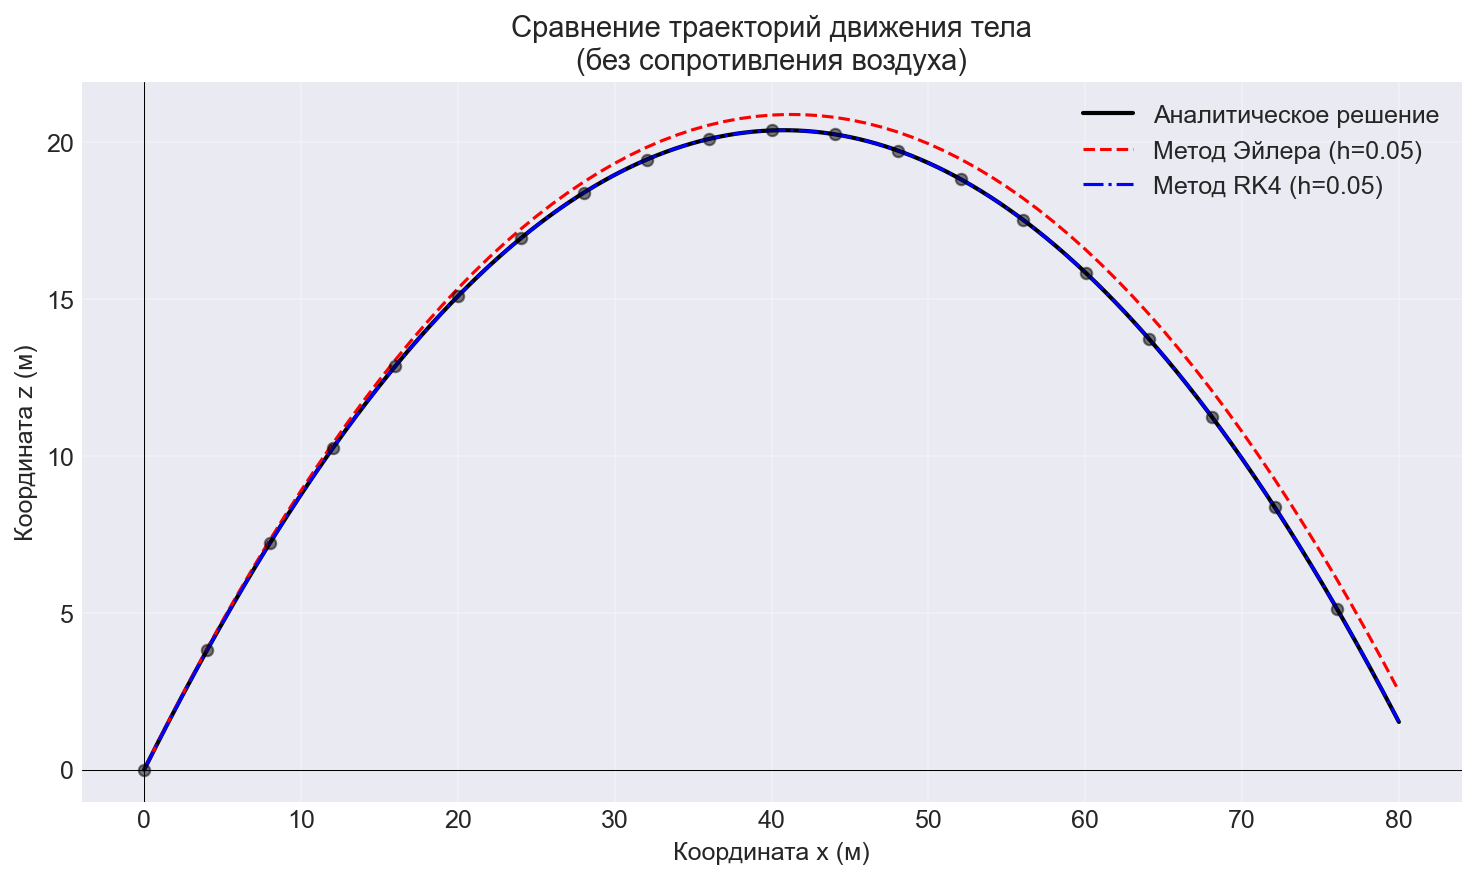
\includegraphics[width=0.7\textwidth]{images/trajectories.png}
\caption{Сравнение траекторий движения тела: аналитическое решение, метод Эйлера, метод RK4}
\label{fig:trajectories}
\end{figure}

На рисунке~\ref{fig:drag} представлено сравнение траекторий с учетом и без учета сопротивления воздуха.

\begin{figure}[H]
\centering
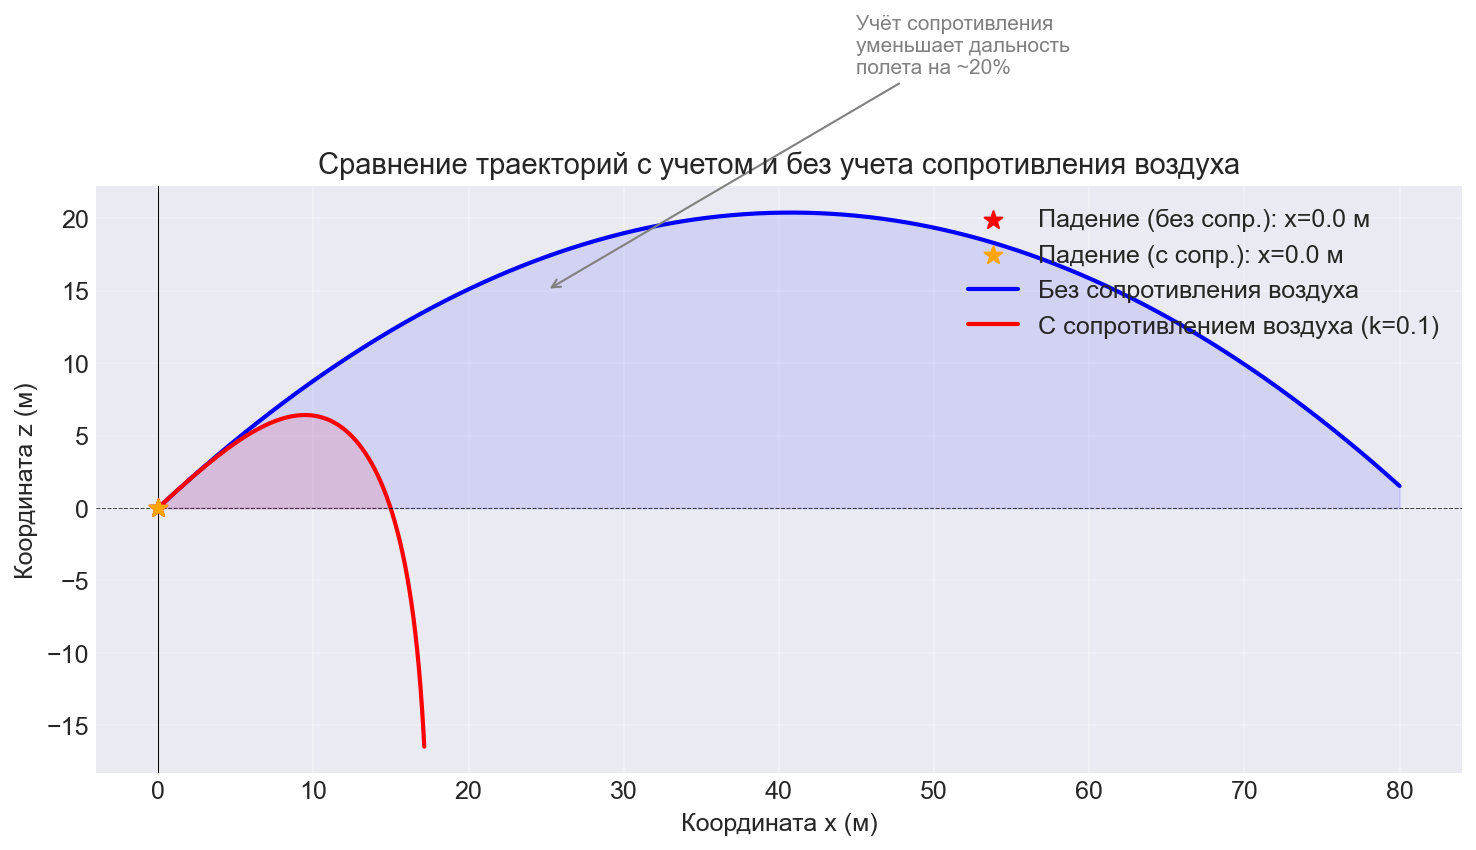
\includegraphics[width=0.7\textwidth]{images/drag_comparison.png}
\caption{Сравнение траекторий с учетом и без учета сопротивления воздуха}
\label{fig:drag}
\end{figure}

\subsection{Анализ результатов}

Проведенное исследование позволяет сделать следующие выводы:

\begin{enumerate}
    \item Метод Эйлера прост в реализации, но обладает низкой точностью и требует очень малого шага интегрирования для получения приемлемых результатов.
    \item Метод Рунге-Кутты 4-го порядка обеспечивает высокую точность при значительно меньших вычислительных затратах.
    \item Учет сопротивления воздуха приводит к существенному изменению траектории: дальность полета уменьшается, траектория становится асимметричной.
    \item Для большинства инженерных задач метод RK4 является оптимальным выбором с точки зрения соотношения точности и вычислительной сложности \cite{bakhvalov2020}.
\end{enumerate}